
\section{Background and Overview}

\label{sec:overview}
%Our method is designed for boolean operations on arbitrary number of regular triangle meshes \cite{requicha1985boolean}. Input meshes are required to be free from self-intersecting, and they are represented with B-reps with geometry connectivity (e.g., halfedge, winged-edge, etc.). Despite of these requirements, our method is robust and not sensitive to topology deficiencies like holes and self-intersections and works correctly if deficiencies are not near the intersection areas between meshes.

Our method is designed for boolean operations on an arbitrary number of regular triangular meshes\cite{requicha1985boolean}. Input meshes are required to be free of self-intersecting regions, and are represented by B-reps with geometric connectivity (for example, half-edge, or winged-edge). Our method is robust and not sensitive to topological deficiencies, such as holes and self-intersections, and works reliably if deficiencies are not near the regions where meshes intersect.


\subsection{Boolean Numerical Errors}
\label{sec:paradigm}

%The boolean operation of triangle meshes is in essence a process of face selection. Namely, given a boolean function, it reserves those primitive faces that pass the function and drop the others to generate the final mesh. Unfortunately, for B-rep meshes, not all the input faces can be classified as a whole, since for faces near the intersections, only parts of them belong to the final mesh. Therefore, we need an extra step aiming at detecting intersections between meshes and performing tessellation. Most of the boolean operation methods follow this two-step paradigm, which consists of intersection computation and face classification. So is our method.

The boolean operation on triangular meshes is, in essence, a process of face selection. Namely, given a boolean function, the operation preserves those primitive faces that pass the function, and drops the others to generate the final mesh. Unfortunately, for B-rep meshes, not all of the input faces can be classified collectively, since only parts of the faces near the intersections belong to the final mesh. Therefore, an extra step is required to detect intersections between meshes and perform tessellations. Most of the existing boolean operation methods follow this two-step paradigm; as does our method.

%The first step is intersection computation. Input faces are tested in pairs to compute their intersections. Each input meshes are tessellated according to the intersection results, making every face be completely inside, outside or on the boundary of other primitives. The tessellated meshes are what we called \emph{intersection-free meshes}. Unfortunately, under fix-precision float-point arithmetic, intersection tests are error-prone: first, degenerate cases of intersection are hard to detect; second, when there are intersections, new vertices are introduced into the geometry, whose coordinates cannot be exactly represented by fix-precision float-point numbers.

The first step in our method is computing intersections. Input faces are tested in pairs to determine their intersections. Each of the input meshes are tessellated according to the intersection results, ensuring every face is completely inside, outside, or on the boundary of other primitives. The tessellated meshes are categorized as \emph{intersection-free meshes}. Unfortunately, intersection tests are error prone when fixed-precision floating point arithmetic is used. First, degenerate intersections are hard to detect. Second, intersections introduce new vertices into the geometry, the coordinates of which cannot be exactly represented by fixed-precision floating point numbers.

The second step is face classification. A given face $\bm{s}$ is evaluated to determine whether belongs to the final geometry according to the $n$-primitive boolean function $f$:
%The second step is face classification. A given face s is evaluated to determine whether it belongs to the final geometry, according to the n-primitive boolean function
\begin{equation}
\lambda_f(\bm{s}) = f(\boldsymbol{\Lambda}(\bm{s})) = f(\lambda_1(\bm{s}), \lambda_2(\bm{s}), \cdots, \lambda_n(\bm{s})).
\end{equation}
The parameter $\lambda_i(\bm{s})$ is the space indicator with respect to mesh $M_i$. To compute $\lambda_f(\bm{s})$ and classify $\bm{s}$, the space indicators with respect to all of the primitives ($\boldsymbol{\Lambda}(\bm{s})$) must be known. Each space indicator has four conditions: completely inside (\emph{in}), completely outside (\emph{out}), on the boundary with consistent normals (\emph{same}) or with opposite normals (\emph{oppo}). The rules of boolean function evaluation are described in \cite{douze2015quickcsg,feito2013fast}.

%The parameter ��i(s) is the space indicator with respect to mesh Mi. To compute ��f(s) and classify s, the space indicators with respect to all of the primitives (��(s)) must be known. Each space indicator has four conditions: completely inside (in), completely outside (out), on the boundary with consistent normals (same), or with opposite normals (oppo). The rules of boolean function evaluation are described in [8], [10].

\begin{figure}[t]
\centering
\includegraphics[width=2.2in]{boolean-01}
\caption{In this 2D view, face $\bm{s}$ (the red line segment) of mesh $M_2$ is on the surface of mesh $M_1$. However, because the face barycenter $\bm{v}_{c(\bm{s})}$ is used to compute the indicator, the coordinates of which contain round-off errors, the point could be moved to $\bm{v'}_{c(\bm{s})}$. Thus, $\bm{s}$ may be falsely classified as being outside of $M_1$.}
%In this 2D view, face s (the red line segment) of mesh M2 is on the surface of mesh M1. However, because the face barycenter vc(s) is used to compute the indicator, the coordinates of which contain round-off errors, the point could be moved to vc0(s). Thus, s may be falsely classified as being outside of M1.
\label{fig:falseclass}
\end{figure}

%Face classification also suffers from numerical errors. Many methods classify face according to the indicators of its barycenter using point-in-polyhedron test \cite{feito2013fast,campen2010exact}. However, coordinates of barycenters cannot be exactly represented and could generate false classification (illustrated in Fig. \ref{fig:falseclass}). What makes the problem worse is that for the large amount of faces and input meshes, many methods \cite{pavic2010hybrid,feito2013fast,ogayar2015deferred,zhou2016mesh} take the benefits of the local coherence of indicators, classifying neighboring faces together . Despite of the performance improvement, it can propagate false classification to neighboring faces and lead to wide-range failure.

Face classification is also prone to numerical errors. Many methods classify a face according to the indicators of its barycenter using a point-in-polyhedron test \cite{feito2013fast,campen2010exact}. However, the coordinates of barycenters cannot be exactly represented, and can cause incorrect classifications (Fig. \ref{fig:falseclass}). This problem is often exacerbated by large inputs (faces and meshes), because many methods \cite{pavic2010hybrid,feito2013fast,ogayar2015deferred,zhou2016mesh} rely on the local coherence of the indicators, so classify neighboring faces together. This can improve performance, but can also propagate false classifications to neighboring faces and lead to broader failures.


\subsection{Plane-based Geometry}

\label{sec:substrates}


\begin{wrapfigure}{r}[0in]{0in}
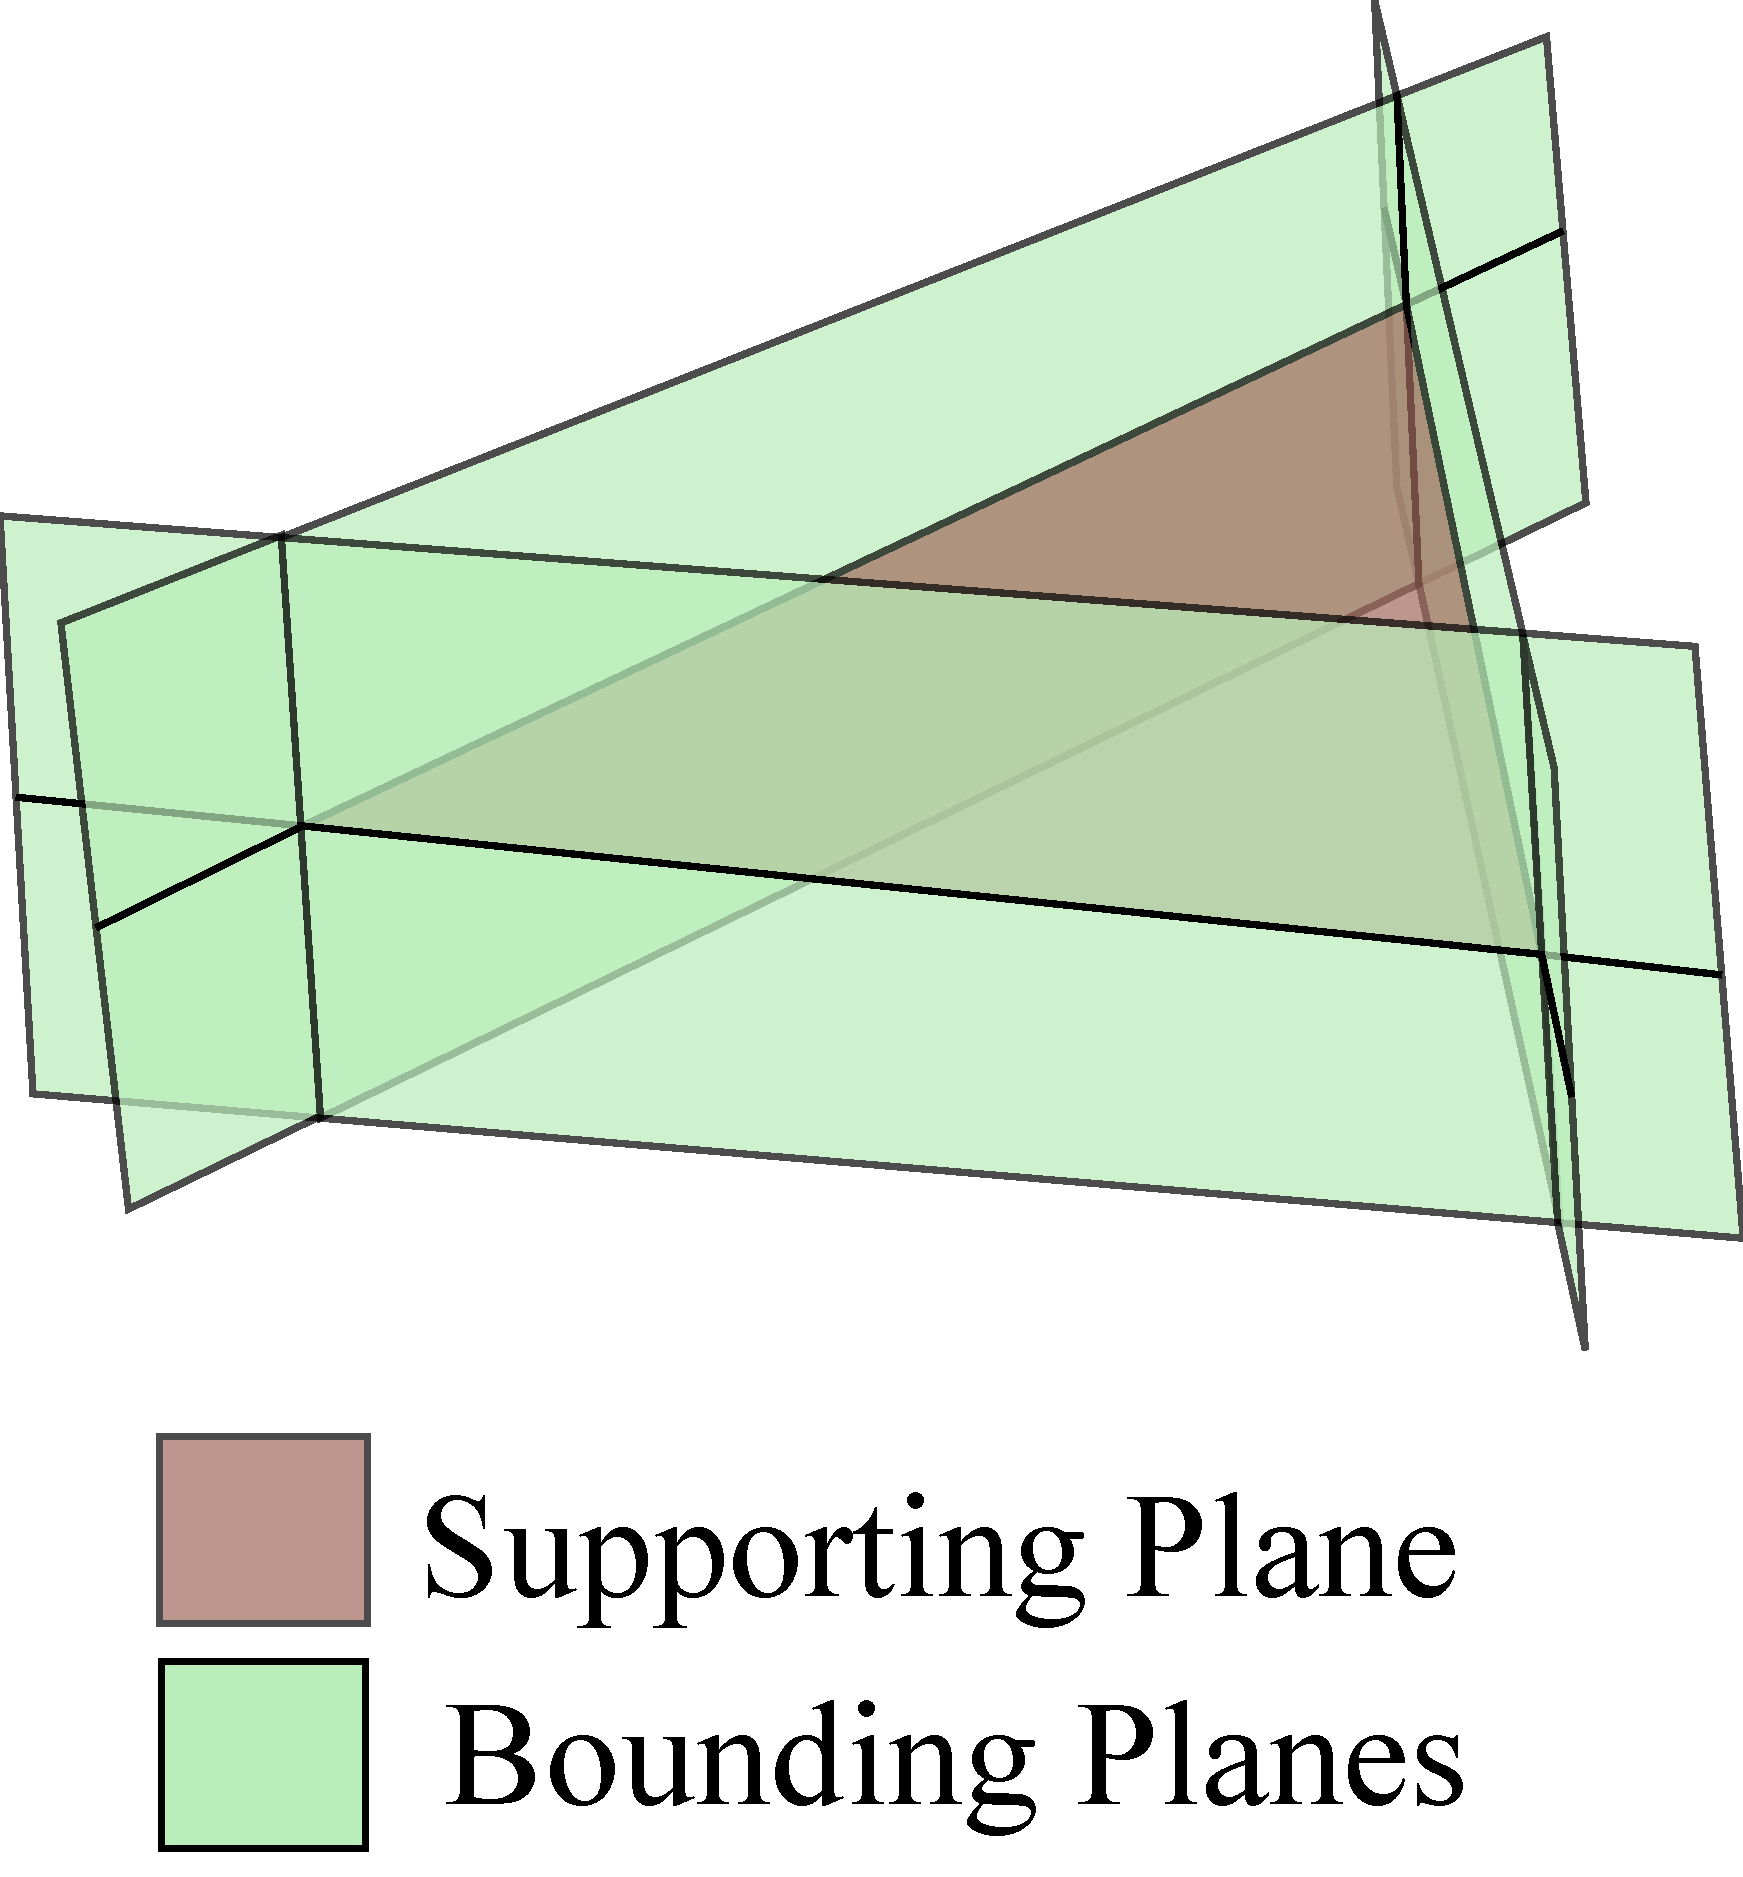
\includegraphics[width=1.5 in]{p-reps}
%\caption{Plane-based representation of triangle}
\end{wrapfigure}

In our method, we avoid numerical errors by embedding P-reps into conventional B-rep boolean algorithms and substituting constructions using B-reps with predicates using P-reps. Using P-reps, each face $\bm{s}$ with $n$ edges is represented by a supporting plane $\bm{p}_{s,sp}$ on which the face lies, and a set bounding planes $\{\bm{p}_{s,b}^i \ \vert\  i = 0, 1,...,n-1\}$. Each edge line $\bm{e}_{\bm{s}}^i$ is represented by the intersection $\bm{p}_{s,sp} \cap \bm{p}_{s,b}^i$. Corner vertex $\bm{v}_s^i$ is represented by $\bm{p}_{s,sp} \cap \bm{p}_{s,b}^i \cap \bm{p}_{s,b}^{{(i+1)}\bmod{n}}$. We use the method of Campen et al. \cite{campen2010exact} for the exact conversion of triangles to their P-reps. All geometric predicates are computed using filtering techniques proposed by Shewchuk \cite{shewchuk1997adaptive}, for both exactness and efficiency.

%In our method,

Other commonly used notations in this paper are presented here. The normal of a plane $\bm{p}$ is denoted as $\bm{n}(\bm{p})$. A line $\bm{l}$ can be represented by the intersection of two planes $(\bm{p}_l^0 \cap \bm{p}_l^1)$, hence, $\bm{l}\colon(\bm{p}_l^0 \cap \bm{p}_l^1)$. The positive direction of the line $\bm{l}$ is defined by $\bm{n}(\bm{p}_l^0) \times \bm{n}(\bm{p}_l^1)$. A point $\bm{v}$ can be represented by non-trivial plane triples $(\bm{p}_v^0 \cap \bm{p}_v^1 \cap \bm{p}_v^2)$, hence, $\bm{v}\colon(\bm{p}_v^0 \cap \bm{p}_v^1 \cap \bm{p}_v^2)$.

%Other commonly used notations in this paper are presented here.


%Plane-based geometry predicates used in our method are mostly well-discussed in previous work \cite{bernstein2009fast,banerjee1996topologically}. In the following, we focus on two predicates related to sorting, which are designed for our method particularly.

The plane-based geometric predicates used in our method have mostly been discussed thoroughly in previous work \cite{bernstein2009fast,banerjee1996topologically}. In the following sections, we focus on two predicates related to sorting, which were specifically designed for our method.

\vspace{0.5em}
\noindent \textbf{Linear ordering of points}

\begin{figure}
  \centering
  % Requires \usepackage{graphicx}
  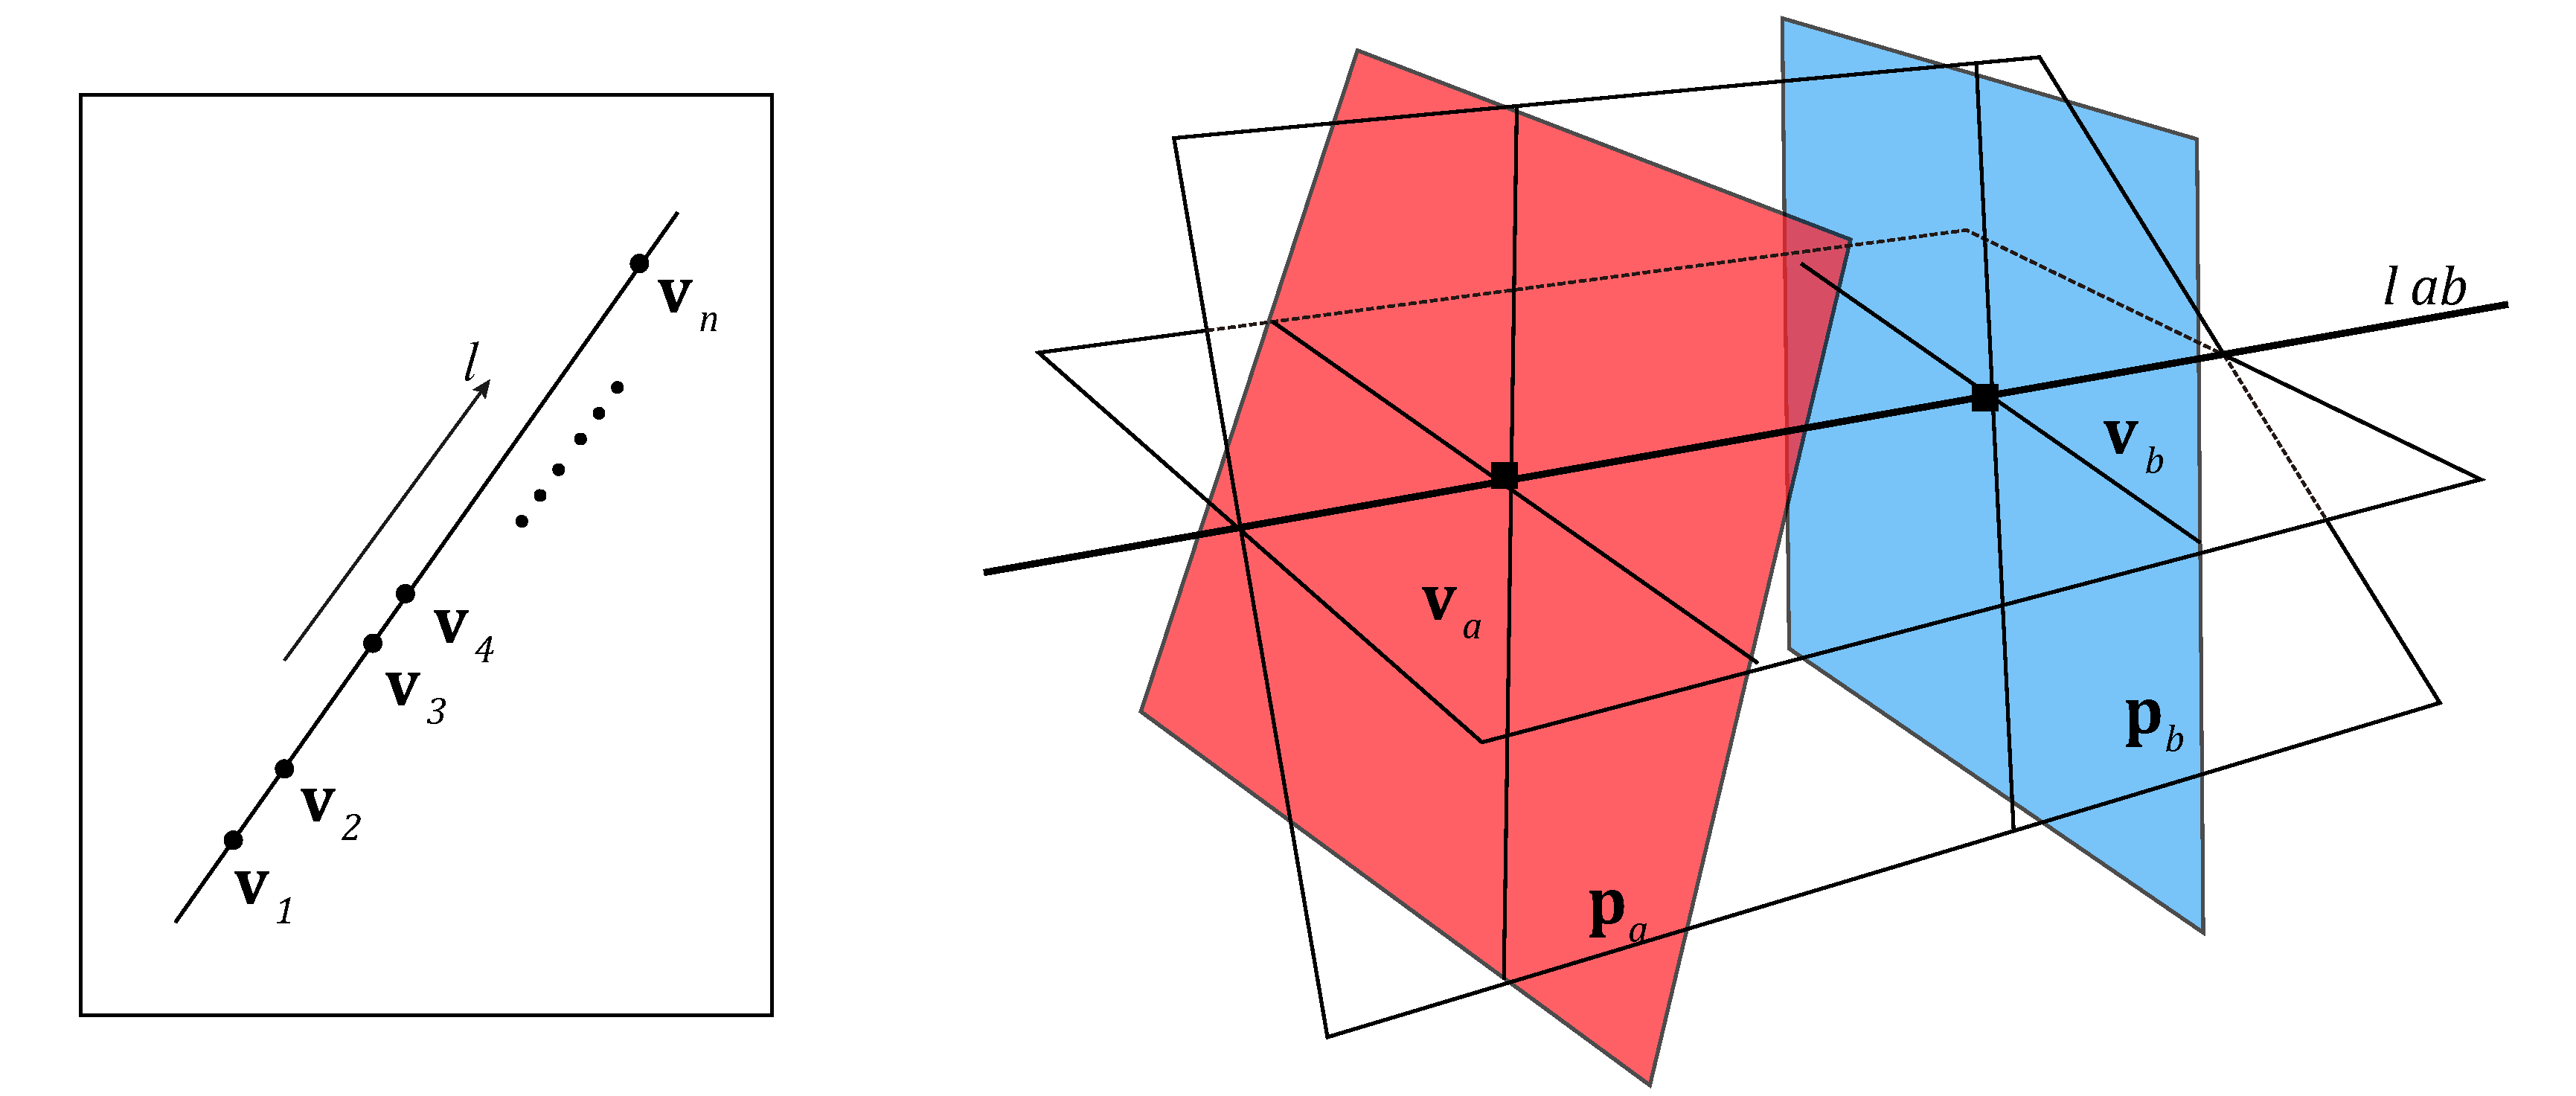
\includegraphics[width=3.5in]{twopointoneline}\\
  \caption{Geometric configuration of the linear ordering of points. Points $\bm{v}_a$ and $\bm{v}_b$ are both on line $\bm{l}_{ab}$. We convert this problem into the plane ordering of $\bm{p}_a$ and $\bm{p}_b$ along $\bm{l}_{ab}$.}\label{fig:twopointoneline}
  %Geometric configuration
\end{figure}


%\noindent Given an line $\bm{l}_{ab}$ with two points $\bm{v}_a\colon(\bm{p}_a^0\cap\bm{p}_a^1\cap\bm{p}_a^2)$ and $\bm{v}_b\colon(\bm{p}_b^0\cap\bm{p}_b^1\cap\bm{p}_b^2)$ on it, we need to determine the linear order of the two points along $\bm{l}_{ab}$ (Fig. \ref{fig:twopointoneline}). To solve this problem, we choose one plane not parallel with $\bm{l}_{ab}$ from the plane representation of each point and convert this problem into linear order of planes, which can be solved by Banerjee et al.'s method \cite{banerjee1996topologically}. The chosen planes should have the same orientation with $\bm{l}_{ab}$ (the dot product between plane normal and $\bm{l}_{ab}$ has to be positive) and unqualified planes have %to be flipped.

\noindent Given a line $\bm{l}_{ab}$ with two points on it, $\bm{v}_a\colon(\bm{p}_a^0\cap\bm{p}_a^1\cap\bm{p}_a^2)$, and $\bm{v}_b\colon(\bm{p}_b^0\cap\bm{p}_b^1\cap\bm{p}_b^2)$, we need to determine the linear order of the two points along $\bm{l}_{ab}$ (Fig. \ref{fig:twopointoneline}). To solve this problem, we choose one plane that is not parallel with $\bm{l}_{ab}$ from the plane representation of each point, then convert this problem into one of determining the linear order of planes, which can be solved using the method of Banerjee et al. \cite{banerjee1996topologically}. The chosen planes should have the same orientation with respect to $\bm{l}_{ab}$ (the dot product between the plane normal and $\bm{l}_{ab}$ must be positive); unqualified planes need to be flipped.


\begin{wrapfigure}{r}[0in]{0in}
\includegraphics[width=1.5 in]{boolean-02}
\end{wrapfigure}
\vspace{0.5em}
\noindent \textbf{Circular ordering of lines}~~~~

%\noindent During face tessellation, we need to know which edges are neighbors (Fig. \ref{fig:circularorder}). This requires circular ordering of directed lines around a vertex. Lines can be sorted in a divide-and-conquer way based on the relative order of each pair of lines. Thus, this problem is converted to one where given two lines $\bm{l}_a$ and $\bm{l}_b$ in a plane $\bm{p}_0$ and their intersection point $\bm{v}_{ab}$, compute the circular order of the two lines. We can compute the order by the sign of $\sin{\theta_{ab}}$, where $\theta_{ab}\in(-\pi,\pi)$ is the angle from $\bm{l}_a$ to $\bm{l}_b$ under the top view of $\bm{p}_0$. The sign of $\sin{\theta_{ab}}$ is the same as triple product $\bm{n}(\bm{p}_0) \cdot (\bm{l}_a\times\bm{l}_b)$. However, explicit computing this equation is complicated because both $\bm{l}_a$ and $\bm{l}_b$ are implicitly represented by intersection of planes.
\noindent During face tessellation, we need to know which edges are neighbors (Fig. \ref{fig:circularorder}).  This requires circular ordering of directed lines around a vertex. Lines can be sorted in a divide-and-conquer way, based on the relative order of each pair of lines. Thus, this problem is converted to one where, given two lines $\bm{l}_a$ and $\bm{l}_b$ in a plane $\bm{p}_0$ and their intersection point $\bm{v}_{ab}$, circular order of the two lines needs to be computed.
We can compute the order by the sign of $\sin{\theta_{ab}}$, where $\theta_{ab}\in(-\pi,\pi)$ is the angle from $\bm{l}_a$ to $\bm{l}_b$ in the top-view of $\bm{p}_0$. The sign of $\sin{\theta_{ab}}$ is the same as the triple product $\bm{n}(\bm{p}_0) \cdot (\bm{l}_a\times\bm{l}_b)$. However, directly computing this equation is complicated, because both $\bm{l}_a$ and $\bm{l}_b$ are implicitly represented by the intersection of planes.

We developed a simpler that requires no explicit computation of $\bm{l}_a$ and $\bm{l}_b$. First, we write the P-reps of the two lines as $\bm{l}_a\colon(\bm{p}_0\cap\bm{p}_a)$ and $\bm{l}_b\colon(\bm{p}_0\cap\bm{p}_b)$. We then orthogonally decompose $\bm{n}(\bm{p}_a)$ and $\bm{n}(\bm{p}_b)$ along $\bm{n}(\bm{p}_0)$:
%We developed a simpler method that requires no explicit computation
\begin{equation}
\begin{split}
&\bm{n}(\bm{p}_a)= \bm{n}^\parallel(\bm{p}_a) + \bm{n}^\perp(\bm{p}_a)\\
&\bm{n}(\bm{p}_b)= \bm{n}^\parallel(\bm{p}_b) + \bm{n}^\perp(\bm{p}_b)
\end{split}
\end{equation}
Here superscript `$\parallel$` refers to the projection on $\bm{p}_0$ and `$\perp$` means orthogonal to $\bm{p}_0$. As we know that $\bm{n}^\perp(\bm{p}_a)$ and $\bm{n}^\perp(\bm{p}_b)$ are both parallel to $\bm{n}(\bm{p}_0)$, we get:
%Here superscript ��k�� refers to the projection on p0,
\begin{equation}
\label{eq:circ1}
\bm{n}(\bm{p}_0) \cdot (\bm{n}(\bm{p}_a) \times \bm{n}(\bm{p}_b)) = \bm{n}(\bm{p}_0) \cdot (\bm{n}^\parallel(\bm{p}_a) \times \bm{n}^\parallel(\bm{p}_b)).
\end{equation}
By observation we find that the angle between $\bm{n}^\parallel(\bm{p}_a)$ and $\bm{n}^\parallel(\bm{p}_b)$ is exactly $\theta_{ab}$. Therefore the sign of the right side of equation \ref{eq:circ1} is exactly the sign of $\sin{\theta_{ab}}$. Thus, we come to the following conclusion:
%By observation, we find that the angle between
\begin{equation}
\label{eq:circ2}
sign(\sin{\theta_{ab}})=  sign(\bm{n}(\bm{p}_0)\cdot(\bm{n}(\bm{p}_a) \times \bm{n}(\bm{p}_b)))
\end{equation}

%Since all the three vectors on the right side are already explicitly represented, we only have to evaluate the sign of an 3$\times$3 matrix and avoid complicated arbitrary precision float-point arithmetic.
As the three vectors on the right side are already explicitly represented, we only need to evaluate the sign of a 3$\times$3 matrix, which avoids complicated arbitrary precision floating point arithmetic.

\begin{figure}[t]
\centering
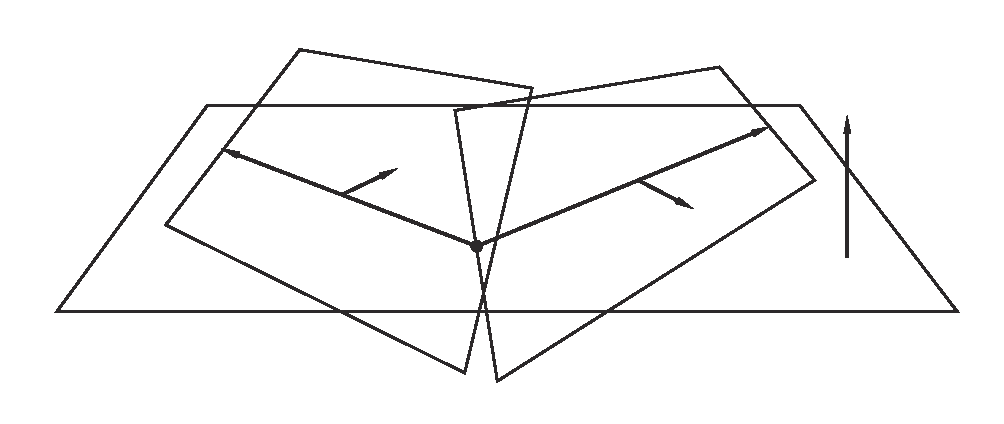
\includegraphics[width=3.5in]{circularorder}
\caption{Geometric configuration of the circular ordering of lines. $\bm{l}_a\colon(\bm{p}_0 \cap \bm{p}_a)$ and $\bm{l}_b\colon(\bm{p}_0 \cap \bm{p}_b)$ are within plane $\bm{p}_0$.}
%Geometric configuration of the circular ordering of lines. la:
\label{fig:circularorder}
\end{figure}


\subsection{Method Overview}


%There are generally three steps in our method. The first step is to compute intersections between each triangle face pairs. After that, the input meshes are tessellated into intersection-free meshes according to these intersections. The last step is to classify each face and generate the final result mesh.

There are three steps to our method. The first step is to compute the intersections between each triangle face pair. In the second step, the input meshes are tessellated into intersection-free meshes according to these intersections. Lastly, each face is classified and the final mesh is generated.

\subsubsection{Intersection computation}

%In this step, we only compute intersections between triangle pairs. The triangle-triangle intersection test is largely based on M\"{o}ller's algorithm \cite{moller1997fast} for its efficiency. However, conventional implementation of M\"{o}ller's algorithm using vertex-based geometry brings numerical errors. Therefore, we integrate P-rep into M\"{o}ller's algorithm. All intersection points and line segments are represented using planes to avoid explicitly computing the coordinates. Also, we carefully deal with degenerate cases of triangle intersections, including point intersections, edge intersections and coplanar situations. In addition, octree is used to speed up the whole process. Details are provided in \S\ref{section:isect}.

In this step, we only compute the intersections between pairs of triangles. The triangle-triangle intersection test is largely based on M\"{o}ller��s algorithm \cite{moller1997fast}, because of its efficiency. However, the conventional implementation of M\"{o}ller��s algorithm using vertex-based geometry introduces numerical errors. Therefore, we integrate P-reps into M\"{o}ller��s algorithm. All intersection points and line segments are represented using planes, to avoid explicit computation of the coordinates. In addition, we carefully deal with degenerate cases of triangle intersections, including point intersections, edge intersections, and coplanar situations. Furthermore, octree is used to speed up the process. Details are provided in \S\ref{section:isect}.

\subsubsection{Deferred tessellation}

%Once all intersections between triangles are detected, we need to tessellate the input meshes and construct the intersection-free meshes. In many methods like \cite{ogayar2015deferred}, constraint Delaunay triangulation (CDT) is applied to perform tessellation. However, for a CSG with more than two meshes, intersections may overlap or intersect with each other, and cannot be used for constraints of CDT directly. In addition, as our intersections are represented by planes, implementation of CDT are complex and inefficient, as most CDT algorithms (e.g. \cite{chew1989constrained}, \cite{de1992line}) is not designed to handle planes and requires explicit coordinates. Therefore, we first perform intersection refinement to resolve intersecting intersections. After that, we construct a graph-like structure suitable for P-rep intersections, called \emph{tess-graph}, to guide the exact tessellation of each face. After all faces are tessellated, we get our intersection-free meshes. Details are shown in \S\ref{sec:tessellation}.

Once all of the intersections between triangles are determined, it is necessary to tessellate the input meshes and construct the intersection-free meshes. In many existing methods, such as \cite{ogayar2015deferred}, constrained Delaunay triangulation (CDT) is used to perform tessellations. However, in a CSG with more than two meshes, intersections may overlap or intersect with each other, so cannot be used directly as CDT constraints. In addition, as intersections are represented in our method by planes, implementing CDT would be complex and inefficient, as most CDT algorithms (such as those in \cite{chew1989constrained}, \cite{de1992line}) are not designed to handle planes and instead require explicit coordinates. Therefore, we first perform intersection refinement to resolve overlapping intersections. We then construct a graph-like structure suitable for P-rep intersections, called a \emph{tess-graph}, to guide the exact tessellation of each face. Once all of the faces are tessellated, we obtain intersection-free meshes. Details are given in \S\ref{sec:tessellation}.

\subsubsection{Face classification}

%This step is to choose faces from the intersection-free meshes to generate the final mesh. However, literally computing the indicator vector of each face is unacceptably slow for large CSGs. We utilize the geometry connectivity stored in B-reps to propagate indicators in a flood-filling manner. In addition, many methods use barycenters of faces together with point-in-polyhedra test for face classification, which is not exact nor robust with fix-precision float-point arithmetics. Different from them, we classify faces based on the classification results of exactly represented vertices, including input vertices and newly introduced intersection vertices, and carefully deal with coplanar conditions to ensure topology consistency. Details will be shown in \S\ref{sec:classification}.

The purpose of this step is to choose faces from the intersection-free meshes to generate the final mesh. However, literally computing the indicator vector of each face is unacceptably slow for large CSGs. We utilize the geometric connectivity information stored in B-reps to propagate indicators in a flood-filling manner. In addition, many methods use the barycenters of faces together with a point-in-polyhedra test for face classification, which is neither exact nor robust with fixed-precision floating point arithmetic. However, our method classifies faces based on the classification of exactly represented vertices, including input vertices and novel intersection vertices, and carefully deals with coplanar conditions to ensure topological consistency. Details are given in \S\ref{sec:classification}.


\begin{figure}[t]
\centering
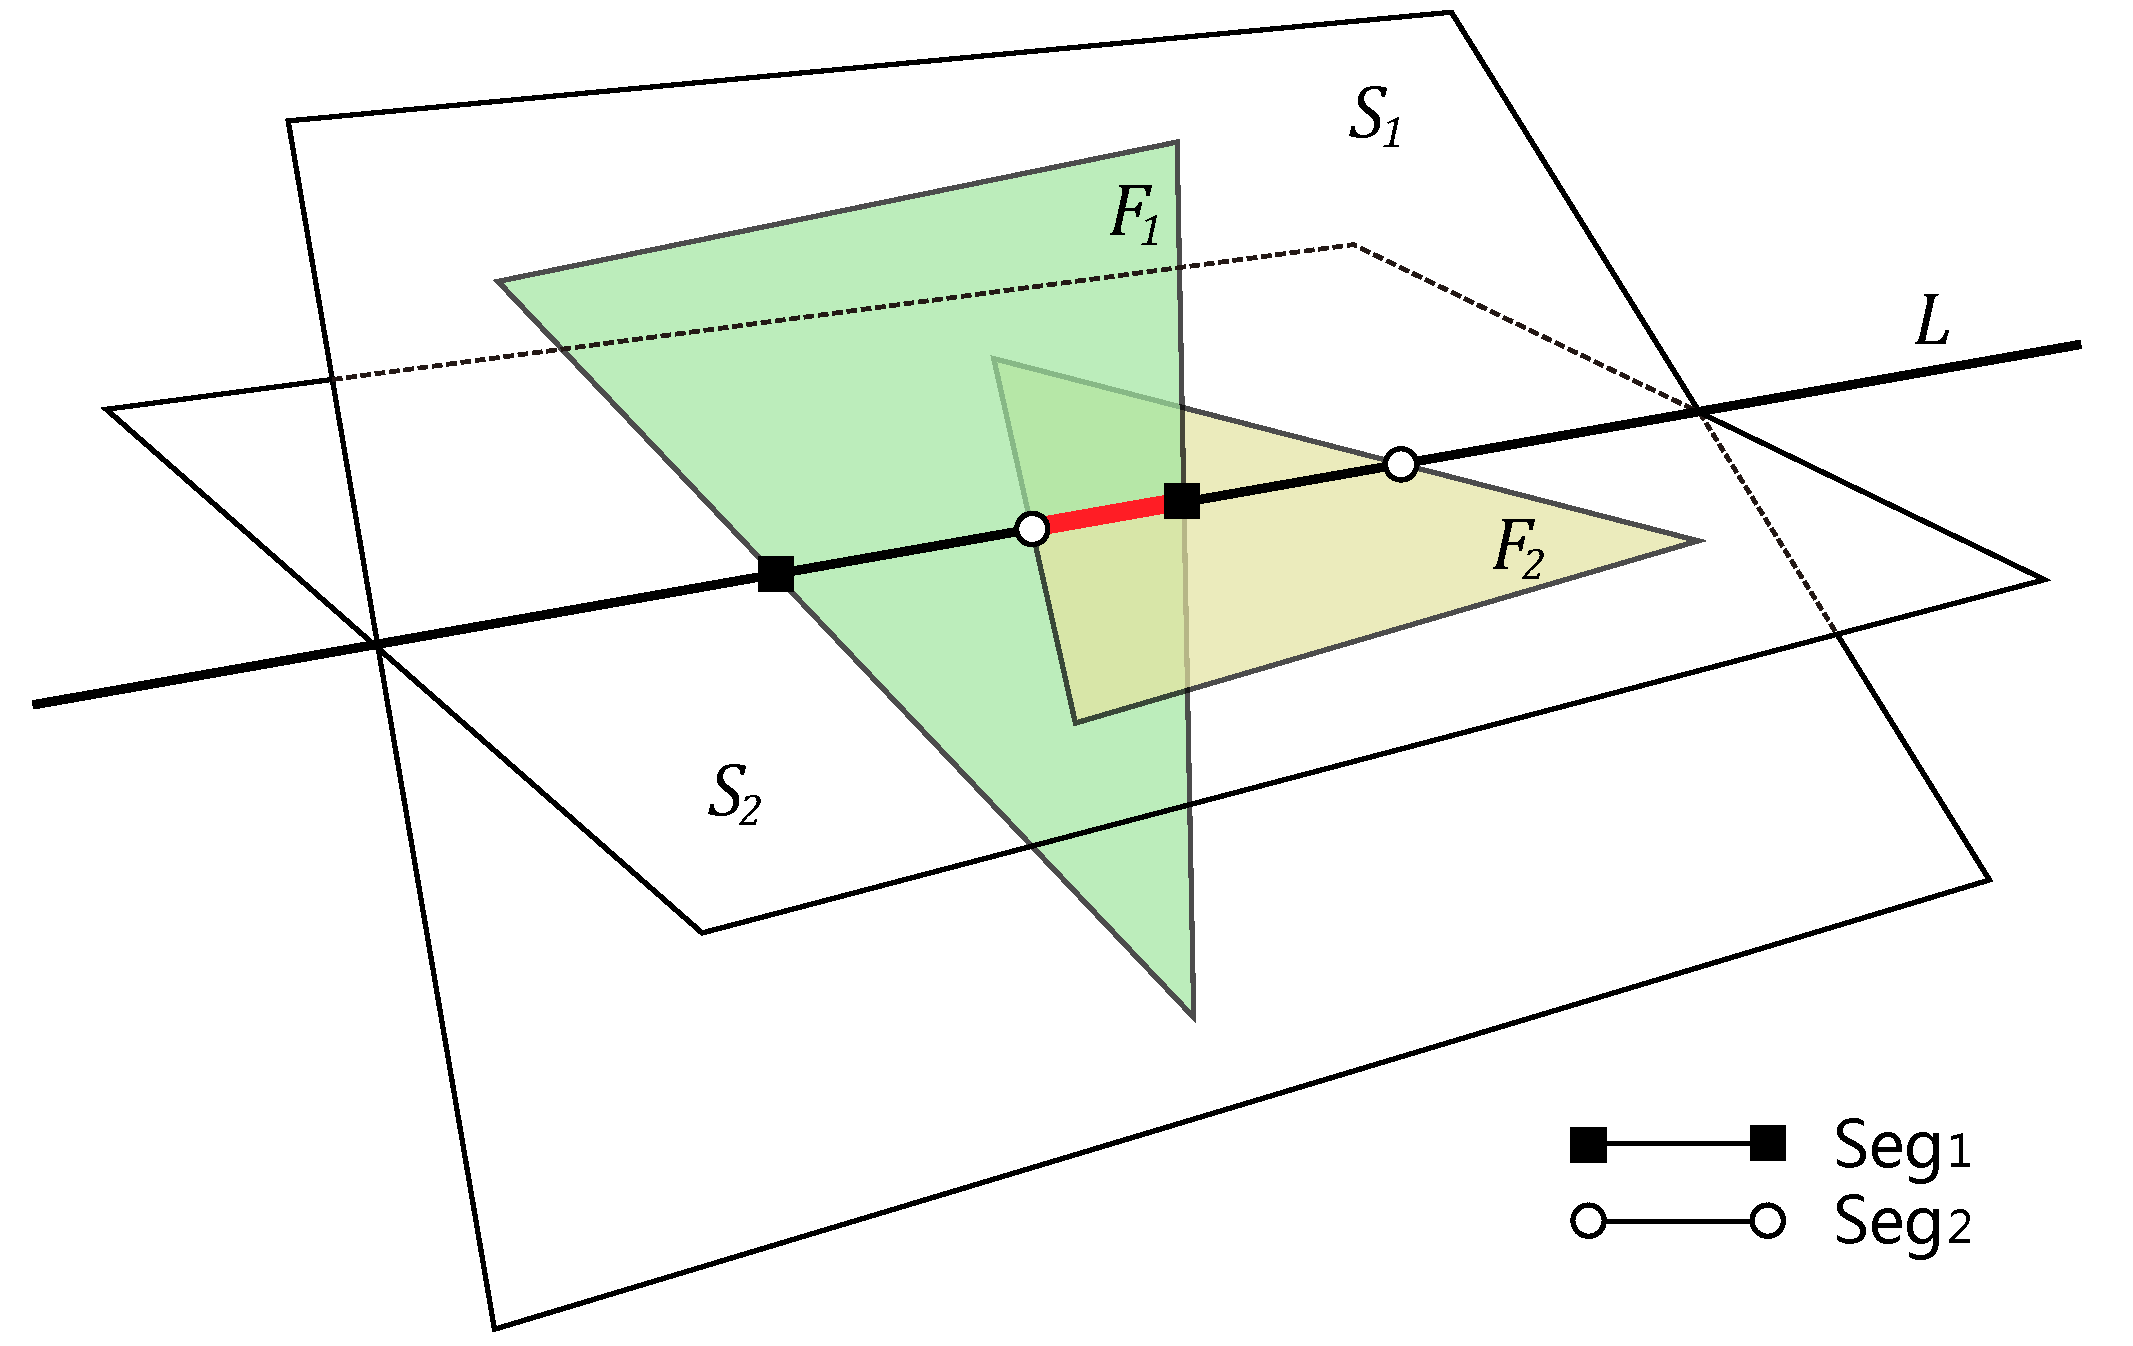
\includegraphics[width=2.5in]{projection}
\caption{$Seg_1$ is the intersection between $\bm{p}_{t_2, sp}$ and $t_1$. $Seg_2$ is the intersection between $\bm{p}_{t_1, sp}$ and $t_2$. The intersection between $t_1$ and $t_2$ (yellow line segment) is the overlap of $Seg_1$ and $Seg_2$.}
%Seg1 is the intersection between pt2,sp and t1. Seg2 is the intersection between pt1,sp and t2. The intersection between t1 and t2 (yellow line segment) is the overlap of Seg1 and Seg2.
\label{fig_projection}
\end{figure}
\section{Intersection Computation}

\label{section:isect}
%In this step, intersections between faces are computed through triangle-triangle intersection test. We adopt M\"{o}ller's algorithm \cite{moller1997fast} on account of its efficiency and simplicity. However, a naive implementation of M\"{o}ller's algorithm can introduce numerical errors and may fail to produce correct results. Therefore, we integrate plane-based geometry to make it exact. In the following, we first introduce our space division strategy to reduce the number of intersection test. Then we make a quick review of M\"{o}ller's algorithm, and discuss the way to embed plane-based geometry. After that, we discuss how to deal with degenerate cases.

In this step, the intersections between faces are determined by a triangle-triangle intersection test. We use  M\"{o}ller��s algorithm \cite{moller1997fast}, because its efficiency and simplicity. However, a na\"{i}ve implementation of  M\"{o}ller��s algorithm can introduce numerical errors, and may fail to produce the correct results. Therefore, we integrate plane-based geometry to ensure the implementation is exact. In the following sections, we introduce our space division strategy to reduce the number of intersection tests. Then we make a quick review of  M\"{o}ller��s algorithm, and discuss how to embed plane-based geometry. Lastly, we discuss how to deal with degenerate cases.



\subsection{Space Division}
\begin{wrapfigure}{r}[0in]{0in}
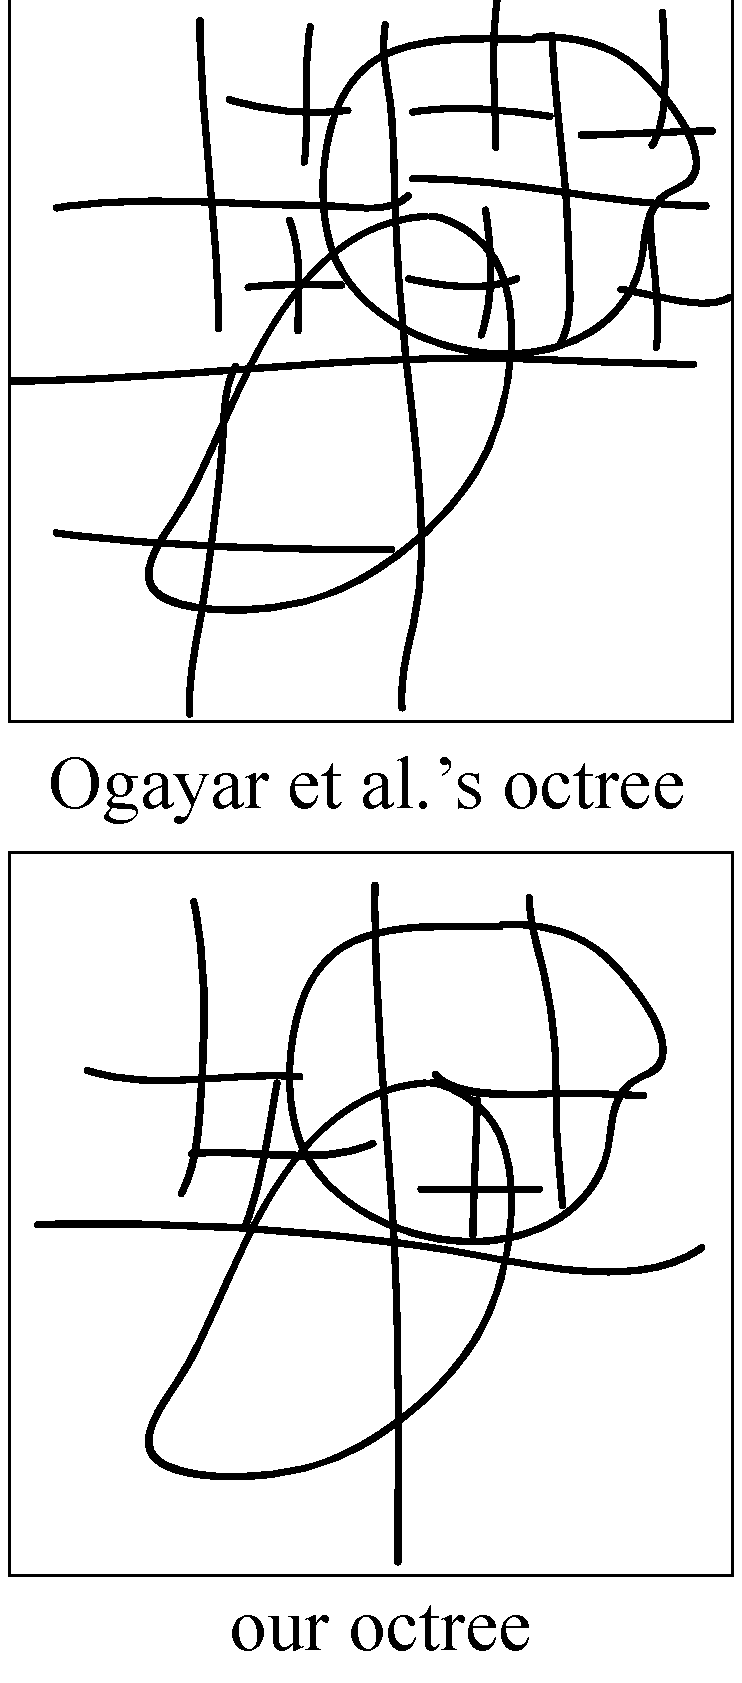
\includegraphics[width=1.2in]{octreediff}
\end{wrapfigure}


%As intersection detection is performed between each pair of faces, localization is necessary for large CSGs to reduce the number of testing pairs. We use the adaptive octree for this purpose. Our implementation is akin to the implementation in Ogayar et al.'s method \cite{ogayar2015deferred}. Intersection between triangle faces and octree nodes are efficiently detected using the separating axis theorem \cite{gottschalk1996obbtree}. Octree leaves are classified into two types: if all faces that intersect a leaf belong to the same mesh, we call it a \emph{normal cell}. Otherwise, it is a \emph{critical cell}, within which the following intersection computation is performed.

As intersection detection is performed between each pair of faces, localization is necessary for large CSGs to reduce the number of pairs to be tested. We use an adaptive octree for this purpose. Our implementation is akin to the implementation of Ogayar et al. \cite{ogayar2015deferred}. The intersections between triangle faces and octree nodes are efficiently detected using the separating axis theorem \cite{gottschalk1996obbtree}. Octree leaves are classified into two types. If all faces that intersect a leaf belong to the same mesh, we regard it as a \emph{normal cell}. Otherwise, it is regarded as a \emph{critical cell}, within which the following intersection computation is performed��

%The difference between our octree and Ogayar et al.'s is that we do not subdivide any normal cell no matter how many faces it contains. This is because subdividing normal cells benefits only the point-in-polyhedron test \cite{frisken2002simple}, which seldom uses in our method. This simplification can save much computing time, especially when intersections between primitives are not complex and located in small regions.

The difference between our octree and that of Ogayar et al. is that we do not subdivide any normal cell, no matter how many faces it contains. Subdividing normal cells is only beneficial for the point-in-polyhedron test \cite{frisken2002simple}, which is seldom used in our method. This simplification saves significant computing time, especially when intersections between primitives are simple, and located in small regions.


\subsection{M\"{o}ller's Vertex-Based Method}



M\"{o}ller's algorithm computes the intersection between two triangles $t_1$ and $t_2$ in three steps as shown in Fig. \ref{fig_projection}:
\begin{itemize}[leftmargin=0.45cm]
\item[1)] An early rejection is performed by testing whether $t_1$ intersects $\bm{p}_{t_2, sp}$, the supporting plane of $t_2$. The same test is also carried out between $t_2$ and $\bm{p}_{t_1, sp}$.
\item[2)]The intersection between $t_1$ and $\bm{p}_{t_2, sp}$, denoted as $Seg_1$, and the intersection between $t_2$ and $\bm{p}_{t_1, sp}$, denoted as $Seg_2$, are computed separately.
 \item[3)]The intersection between $t_1$ and $t_2$ is determined by computing the overlap between $Seg_1$ and $Seg_2$ .
\end{itemize}

%Moller��s algorithm computes the intersection between two triangles t1 and t2 in three steps, as shown in Fig. 4.

%The non-robustness of this algorithm is from computing the coordinates of intersection vertices, which is the end points of $Seg1$ and $Seg2$. Although implementation with arbitrary precision arithmetic produces exact coordinates, it is too costly for boolean operations of large CSG. We use plane-based geometry to solve this problem by implicitly representing intersections with planes.


The non-robustness of this algorithm stems from computing the coordinates of the intersection vertices (the end points of $Seg_1$ and $Seg_2$). Although implementation of this algorithm with arbitrary precision arithmetic produces exact coordinates, it is too costly for boolean operations with large CSGs. We use plane-based geometry to solve this problem, by implicitly representing intersections with planes.
